\documentclass[11.5pt]{sig-alternate}
\usepackage[defaultlines=3,all]{nowidow}
\usepackage{hyperref}
\usepackage{tabularx}
\usepackage{graphicx}
\usepackage{blindtext}
\usepackage[utf8]{inputenc}
\usepackage[english]{babel}
\usepackage{lastpage}
\usepackage{float}
\usepackage{comment}
\usepackage{multicol}
\usepackage{dirtytalk}
\usepackage{xcolor}
\usepackage{hanging}
\usepackage{array,url,kantlipsum}
\usepackage{wrapfig}
\usepackage[backend=biber, style=apa]{biblatex}
\addbibresource{notation.bib}
\usepackage{authblk}
\usepackage{caption}
\usepackage{graphicx,subfigure}
\usepackage{authblk}
\usepackage{enumitem}
\usepackage[utf8]{inputenc}
\usepackage{cuted}
\usepackage{fancyhdr}
\usepackage{multirow}
\pagestyle{fancy}
\usepackage{lipsum}
\usepackage{xurl}
\raggedbottom
\renewcommand{\headrulewidth}{0pt}
\renewcommand{\footrulewidth}{0pt}
\setlength\headheight{80.0pt}
\addtolength{\textheight}{-80.0pt}
\chead{%
  \ifcase\value{page}
  % empty test for page = 0
 \or 
\includegraphics[width=\textwidth]{headerImage.png}% page=1
  \or 
\includegraphics[width=\textwidth]{headerImage.png}% page = 2
  \or 
\includegraphics[width=\textwidth]{headerImage.png}% page = 3
  \or 
\includegraphics[width=\textwidth]{headerImage.png}% page = 4
  \or 
\includegraphics[width=\textwidth]{headerImage.png}% page = 5
  \else
  
\includegraphics[width=\textwidth]{headerImage.png}
  \fi
}

%\chead{
\includegraphics[width=\textwidth]{headerImage.png}}
\fancyfoot[LE,LO]{Program for Neurodivergent Undergraduate STEM Students\\           
DOI: }
\fancyfoot[CE,CO]{{ }}
\fancyfoot[RE,RO]{\thepage}
\pagenumbering{arabic}
\hypersetup{
    colorlinks=true,
    urlcolor=blue
}
 
\let\oldabstract\abstract
\let\oldendabstract\endabstract
\makeatletter
\renewenvironment{abstract}
{\renewenvironment{quotation}%
               {\list{}{\addtolength{\leftmargin}{1em} % change this value to add or remove length to the the default
                        \listparindent 1.5em%
                        \itemindent    \listparindent%
                        \rightmargin   \leftmargin%
                        \parsep        \z@ \@plus\p@}%
                \item\relax}%
               {\endlist}%
\oldabstract}
{\oldendabstract}
\makeatother

% Left align captions
\captionsetup{justification   = raggedright,
              singlelinecheck = false}


\begin{document}

\title{Scholar Perspectives on the Impact of a Scientific Community Program for Neurodivergent Undergraduate STEM Scholars}

\author[1]{\large \color{blue} Dylan Sullivan}
\author[1]{\large \color{blue} Derek Hidalgo}
\author[1]{\large \color{blue} Jacob Stolle}
\author[1]{\large \color{blue} Fernando Zavala}
\author[1]{\large \color{blue} Rebecca Matte}
\author[1]{\large \color{blue} Rebecca Matte}



\affil[1]{Landmark College}
\toappear{}

\maketitle
\begin{@twocolumnfalse} 
\begin{abstract}
\item 
\begin{large}
 \textit{Despite the adaptive strengths and unique problem-solving skills demonstrated by neurodivergent (ND) individuals, they remain marginalized in Science, Technology, Engineering and Mathematics (STEM) fields. High unemployment rates among individuals with disabilities emphasize the need for addressing barriers to entry and persistence in the workforce. This study introduces a program designed to enhance opportunities for neurodivergent STEM scholars with financial needs, supported by the National Science Foundation (NSF). The program involves: 1) a weekly cohort course to engage in professional development, 2) use of the Birkman Method® survey to help scholars identify and communicate strengths, fostering self-awareness and growth, and 3) one-on-one mentoring with STEM faculty and career counselors to assist scholars in identifying and pursuing internship opportunities and developing career paths.}
 
\textit{This paper, co-written by cohort scholars, highlights the program’s successes, to date, in facilitating internships for neurodivergent scholars, addressing challenges associated with executive function, and providing ongoing support through cohort activities and mentorship. Overall, the program seeks to bridge the gap between neurodivergent scholars and STEM opportunities. This paper contains suggestions for program design for neurodivergent STEM scholars from the scholars’ perspectives.}\\
 

  
    
 Keywords: STEM; neurodivergent; neurodiversity; undergraduate; community; sense of belonging
 \end{large}     
\end{abstract}
\end{@twocolumnfalse}

%% ABSTRACT


%% AUTHOR INFORMATION

\textbf{*Corresponding Author, Christin Monroe}\\
\href{mailto:christinmonroe@landmark.edu}{(christinmonroe@landmark.edu)} \\
\textit{Submitted Mon Jan 15 2024}\\
\textit{Accepted Wed Apr 24 2024} \\
\textit{Published Online DATE} \\
\textit{DOI: } \\

\pagebreak
\pagebreak

\vspace{5mm}
\section*{\vspace{140mm}}
\section*{Background}
\subsection*{Definition of Neurodiversity (ND)}
\begin{large}
Neurodiversity (ND) is a social ideal based on a biological fact. The human brain is the most complex thing on earth, and every brain is different. Neurodiversity is about what that should mean. Instead of separating people into normal and abnormal, neurodiversity asks us to accept variation. To us, it means that autism, ADHD, and learning disabilities are valuable forms of humanity that enrich culture. New ideas, insights, and unique ways of viewing the world come from diverse minds. This is a strength. (Landmark College Center for Neurodiversity, n.d.) 

ND scholars have been historically marginalized in Science, Technology, Engineering and Mathematics (STEM) at the postsecondary level \\(Moon, 2011). Unemployment estimates for individuals with disabilities range from 37\% to 63\% (Newman, 2011) and as high as 80\% (Austin, 2017). It is estimated that 10\% of the US workforce is comprised of individuals with disabilities, but only 2\% of STEM professionals report having a disability (Moon, 2011) and ND scholars are likely not being hired in STEM fields at the rates that match their peers. (Ladner, 2015) It has been well documented that many ND individuals have exceptional adaptive strengths (especially in STEM) and unique problem-solving skills because of the challenges they face in traditional learning environments. (Syharat, 2023) ND scholars develop creative problem solving to overcome previous academic challenges. (Austin, 2017) ND individuals also often possess compensatory gifts that can lead to a major advantage. (Eide, 2011) It is also important to note and address the barriers that ND individuals face in entering and persisting in the workforce. (Krzeminska, 2019) Areas of importance to address when working with ND scholars are: 1) mentoring (Brown, 2010) (Christ, 2013) (Patrick, 2013), 2) internship opportunities (Burgstahler, 2009), and 3) peer support and sense of belonging (Dahlstrom-Hakki, 2020). There are many opportunities to develop best practices for supporting ND STEM scholars both academically and professionally. 

Through funding support from the National Science Foundation (NSF), the Access to Innovative Education: STEM- Providing Learning Opportunities and Scholarship for Neurodivergent Scholars (AIE-STEMPLOS) program is \\mapped out in Figure 1. The goal of this program is to increase accessibility opportunities in education and employment for scholars who have demonstrated above average academic success at the intersection of neurodivergence and financial need that are pursuing either a degree in life science or computer science. A major focus of this program is to provide opportunities to engage and empower scholars, while allowing for a balance of autonomy and accountability. (Perrin, 2014)

\begin{figure*}[htb]
    \centering
    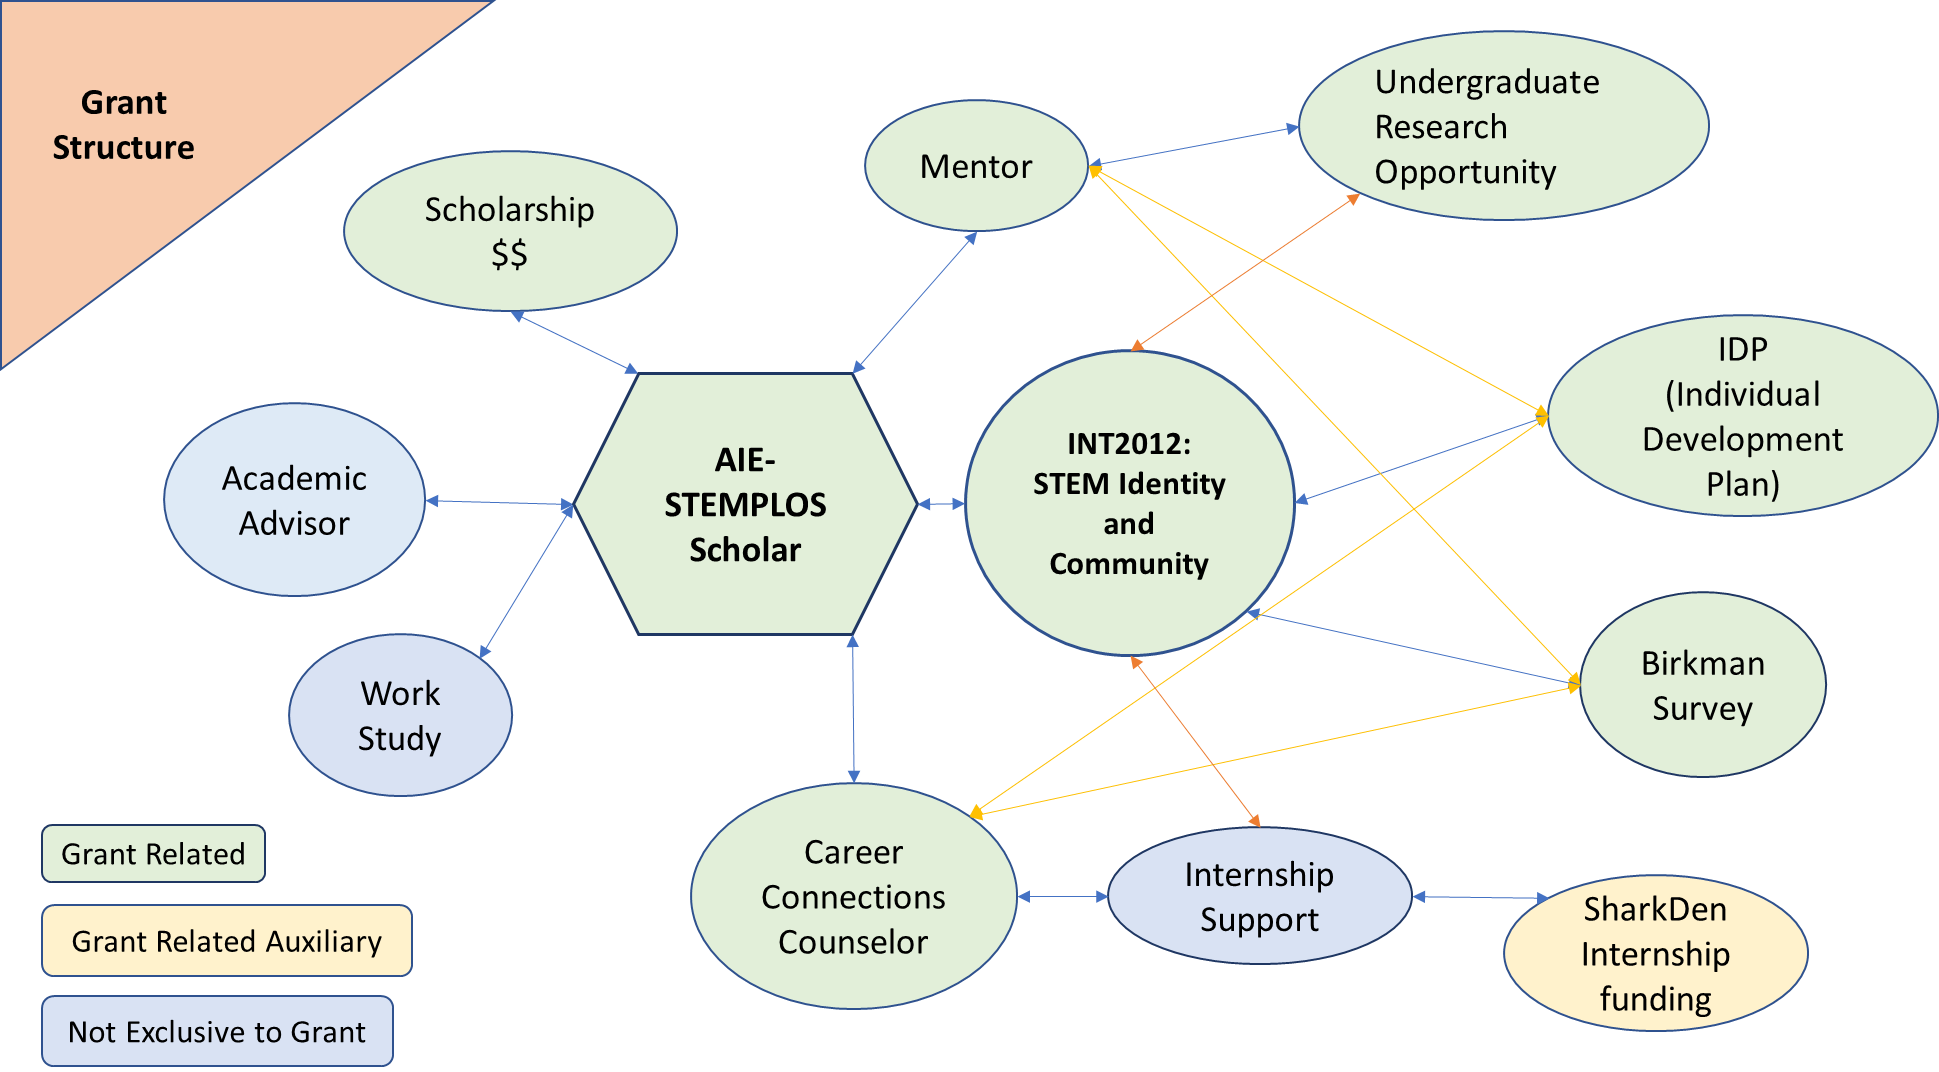
\includegraphics[width=\textwidth]{fig1.png}
     \captionsetup{font=large, labelfont=bf}
    \caption{Map of support provided to STEM scholars.}
    \label{Figure 1}
\end{figure*}

\section*{Methods}
\subsection*{Institutional Review Board (IRB)}
All procedures and materials were approved by a college IRB (\#2020-106).

\subsection*{Participants}

Between Spring 2022 and Fall 2023, twenty-five unique scholars have participated in this program. Four scholars are co-authors on this paper, providing specific feedback about their unique experiences in the program. It is important that neurodivergent scholars share their personal experiences and shape the neurodivergent movement in higher education. (Dwyer, 2023)

\section*{Program Components and Results}
Each of these sections was written by a different scholar in the AIE-STEMPLOS program. Each scholar chose to describe an aspect of the program they found most meaningful. A major goal of this publication is to provide neurodivergent scholars with the opportunity to share their own experiences, in their own words.

\subsection*{Weekly Cohort Course}

To provide scholars with professional development direction, a 1-credit (1-hour) course was created, called STEM Community and Identity. Many ND scholars struggle with executive function challenges, and need dedicated time to prioritize their future, which includes identification of internships. In addition, all scholars receive a \$5,000 scholarship per semester. One of the goals of providing these funds is to lessen the number of hours scholars need to work outside of classes to earn money that is put towards tuition. This course provides scholars with the opportunity to make progress towards the goal of obtaining an internship and utilizing the Birkman® language (see section below for more details) to develop as professionals. Even though the class only meets once a week and tasks are designed to be completed during the class time, the data shows that scholars feel they are always making progress. 

Cohort meetings are calm and comfortable times where scholars can interact with their peers in less intense settings. On average, 88\% of scholars participate in at least 75\% of cohort activities and the program has an 87\% retention rate. The course material is not challenging but is personalized to the scholar. This setting makes scholars excited to attend class and prioritize professional development, which is not always a priority for low-income and neurodivergent scholars who often struggle (for a variety of reasons) with time management.

The course is made up of advanced and novice scholars pursuing an associate or bachelor’s degree in either life science or computer science. The cohort class is “multigenerational,” having novice scholars (new to the program) participate side-by-side with advanced scholars (who have previously participated in the cohort). The advanced scholars (who have completed internships) share their experiences and novice scholars gain insights to real career options (both in terms of subject matter and practical experience). 

Based upon reporting at the end of the semester and scholar enthusiasm, one popular activity takes place each semester where scholars can learn more about their peers is the “Birkman® lineup.” In the Birkman® lineup scholars line up in order of their Birkman ® component scores. This helps scholars better understand themselves and how they are similar and/ or different from their peers.

Each semester, tasks become more complex, and scholars are trained to evaluate themselves professionally before, during and after internship experiences as they develop their balanced disability identities. Scholars create professional language that combines their neurotype with Birkman language. (Gibson, 2006) (Forber-Pratt, 2017)

\section*{Birkman Method®}

The Birkman Method® is a tool used to better understand interpersonal dynamics and achieve higher levels of performance through positive psychology. (Birkman, 2023) Many neurodivergent scholars struggle with identifying and/ or communicating their strengths due to exposure to deficit model philosophies about their perceived disabilities and their personal struggles in traditional academic environments. (Matte, 2023) Scholars are encouraged to make personal decisions about the use of language to describe themselves, their neurodiversity, and whether or not they choose to use the term “disability”. The use of this language is personal and situation dependent. This tool both helps scholars identify and communicate their strengths and provides scholars with information on how one is perceived by others and preferences for how they prefer to be treated.

All scholars, mentors, and career counselors in the program take the Birkman® survey and then are debriefed on the Birkman® survey results with a primary investigator (PI) for this program. To date, 88\% (7/8) mentors and 96\% (24/25) scholars completed the Birkman®. All parties also participate in group activities to better understand how their strengths and stress responses can manifest. The Birkman® language has become a common language for scholars to utilize with mentors and career counselors as they develop professionally. This tool provides an alternative professional language to describe neurodivergence, which includes cognitive, communication and environmental needs.

This tool is revisited regularly throughout the time scholars participate in grant related activities. It provides scholars with language they can employ while developing a professional portfolio (LinkedIn, resume, etc.) and as they both prepare for their internships and reflect on their experiences afterwards.

The benefits of the Birkman Assessment® are increased awareness of strengths, weaknesses, and stresses, along with a better ability to present and express oneself to an employer. The assessment also provides valuable feedback on career path options.

\section*{One-on-One Mentoring and Career Connections}

The role of a mentor and career counselor for each STEM scholar is profound. Mentors can establish and build connections for the scholars assigned to them with career counselors, internships related to science, and people that might be important to a scholar’s career down the road depending on what they plan to do, and much more. A mentor can also be directly involved with an internship depending on the type and location of the internship. More importantly though, a mentor is there to shine a light when a scholar is in the fog about what kind of science career they might excel in, helping them to understand their strengths and identify their interests. The amount of time a mentor spends with a scholar is largely left up to the scholar. A vivid metaphor that is used in the program is that the scholar is the driver of the car and the amount they let the mentor be the backseat driver is under their command. While the importance of mentorship is important for everyone in the program, the involvement of assigned mentor is more important to new recipients of the scholarship compared to advanced students because of the lack of experience, knowledge, and other connections. Early on, mentors need to reach out and show up for their mentees though regular contact to demonstrate their willingness and delight to be a part of the mentees’ journey of growth. If the bond between the scholar and mentor holds strong, a mutually beneficial relationship can lead to amazing results. 

When a recipient joins the grant, they are assigned a career connections counselor. Like the mentor, the career connections counselor can help with identifying internships for work experience. They help scholars with paperwork and resume-building. Once they are told what interests a scholar has, they help look up what kind of workplace would be a realistic fit. Can the scholar drive? What kind of workplace accommodations would the future internee need? Does the scholar require any assistance in communicating with the workplace? It is the career connections counselor’s job to help with all of this and will guide the scholar toward a successful future. 

\section*{Internship Support}

It is not just a matter of financial aid that low-income neurodivergent scholars need to persist in STEM. The process of finding and landing an internship can be an extremely daunting task, and especially so for neurodivergent scholars who might have executive functioning (EF) challenges. Scholars with EF challenges can struggle with “activation energy” to start or persist through long-term or multi-step processes. That means that a neurodivergent scholar with EF challenges while thinking about the total amount of effort it will take for them to complete the tasks associated with landing an internship can be overwhelmed into a state of task paralysis. Even before an attempt is made, no matter whether the scholar is more than capable of completing the work. The process to support the scholar with EF challenges has proved to be beneficial to the entire cohort. The steps of obtaining internships typically involves, 1) identifying internships that are a “good fit”, 2) writing a resume, 3) writing a cover letter, and 4) interviewing. To date, 70\% (11/16) of scholars who have completed this program have participated in internships. This success is found by breaking down each step in the application process into manageable tasks that would usually be self-directed and providing structured support for the scholars. 

It is also important that scholars consider participating in several internships. Such as starting with more in reach internal internships, before moving on to more challenging external internships that may be less structured. It is important to consider the increased self-advocacy that may be required. Ideally, the faculty member serving as the scholar’s mentor may have internship opportunities in which the scholar can participate. Doing internships with trusted mentors, where a relationship has already been established, can allow scholars to feel confident in the application process, and to build confidence before moving onto other opportunities. Scientific research and internships will not always go as planned, but scholars comfortable in an environment are more likely to speak up and contribute, thus building the skills they will need later in STEM.

Scholars participating in external internships are encouraged to stay in touch with their mentors and peers, especially when they encounter difficulties, to help stay on track. Self-advocacy can be a struggle for neurodivergent scholars. Feeling part of a scientific community, reminding the scholars of the unique perspective they have to offer, and having a supportive mentor are all ways to help scholars persevere through the challenges.

The program then asks the scholars after they have completed an internship, to give a presentation on their experience to their peers. The assigned presentation aims to guide personal reflection. This gives the scholars an opportunity to reflect on which aspects of the internships they enjoyed and which they did not. This reflection can inform them about their future career choices. The presentation outline might ask them to answer questions such as, `Were the structures in place conducive to your success?', `In what ways did you advocate for yourself?', `In what ways could you have improved your self-advocacy?'.

Each scholar's presentation also informs their peers what they might consider in their own interning process. Their peers are then given the opportunity to ask the presenting scholar questions and then asked to write down key takeaways from the presentation to serve as a reference for them later. The cohort class then continues to provide support through prioritizing and polishing professional portfolios in a self-sustaining model and serves as a source of accountability for ongoing or future job applications.

\section*{Conclusions}

In conclusion, the presented program, outlined in Figure 1, provides a framework of support to improve access for neurodivergent scholars in STEM careers. Through funding provided by the NSF, the program aims to engage and empower scholars pursuing life science or computer science degrees. Using a scaffolded framework of support including cohort building, mentoring, internship opportunities, and peer support, the program has successfully placed 70\% (11/16) of scholars in internships, compared to only 52\% (11/21) in the previous round of the grant without the cohort class and Birkman® method. The Birkman® has been implemented as a valuable tool for self-awareness and effective communication, fostering a common \\strengths-based language among scholars, mentors, and career counselors. The program's success, to date, is evidenced by these positive outcomes. 

This paper not only highlights the challenges faced by neurodivergent individuals, from their own perspective as co-authors, but also presents tangible and effective programmatic tools that contribute to creating a supportive environment for their academic and professional endeavors in STEM fields. This program provides ongoing support, professional development, and the cultivation of a community that recognizes and values the unique perspective neurodivergent scholars bring to the scientific landscape.

\section*{Acknowledgements}

The authors would like to thank Dr. Brian Young and Dr. Shell Wallace for their input on this project. In addition, we would like to thank Landmark College's Career Connections office for continued support of students in this program. This material is based upon work supported by the National Science Foundation under Grant No 2129912.

\clearpage
\section*{References}\par 

\leftskip 0.25in
\parindent -0.25in 
%%%

Austin, R. \&. (2017). Neurodiversity as a competative edge. \textit{Harvard Business School Review}, 96-103.

Birkman. (2023, 12 31). \textit{Birkman}. Retrieved from About Birkman: Our History and Culture: \url{https://birkman.com/about-birkman#:~:text=Birkman%2C%20The%20Birkman%20Method%20remains,management%2C%20and%20organizational%20design%20today.}

Brown, S. T. (2010). Mentoring individuals with disabilites in postsecondary education: A review of the literature. \textit{Journal of postsecondary education and disability}, 98-111.

Burgstahler, S. (2009). Differences in perceived benefits of internships for subgroups of students with disabilities. \textit{Journal of Vocational Rehabilitation}, 155-165.

Christ, B. (2013). The importance of faculty-student connection in STEM diciplines: A literature review. \textit{Journal of STEM Education}, 22-26.

Dahlstrom-Hakki, I. A. (2020). Comparing synchronous and asynchronous online discussions for students with disabilities: The impact of social presence. \textit{Computers and Education}, 103842.

Dwyer, P. M. (2023). Building neurodiversity-inclusive postsecondary campuses: recommendations for leaders in higher education. \textit{Autism in Adulthood}, 1-14.

Eide, B. E. (2011). \textit{The dyslexic advantage: Unlocking the hidden potential of the dyslexic brain}. London, England: Plume Publishing.

Forber-Pratt, A. J. (2017). Disability Identity Development: A systematic review of the literature. \textit{Rehabilitation psychology}, 198.

Gibson, J. (2006). Disability and Clinical Competency: An introduction. \textit{The California Psychologist} , 6-10.

Krzeminska, A. A. (2019). The advantages and challenges of neurodiversity employment in organizations. \textit{Journals of Management \& Organization}, 453-463.

Ladner, R. B. (2015). Broadening Participation: Increasing the participation of individuals with disabilites in computing. \textit{Communications of the ACM}, 33-36.

Landmark College Center for Neurodiversity. (n.d.). \textit{Center of Neurodiverstiy}. Retrieved from Landmark College: \url{https://www.landmark.edu/center-for-neurodiversity}

Matte, R. (2023, March 16). Strengths-Focused Education for Neurodivergent Students: a conversation. (M. Dipietro, Interviewer)

Moon, N. U. (2011). Evaluation of programmatic interventions to improve postsecondary STEM education for students with disabilities: Findings from SciTrain University. \textit{Journal of Postsecondary Education and Disability}, 331-349.

Newman, L. W.-M. (2011). The post-high school outcomes of young adults with disabilities up to 8 years after high school. \textit{A report from the National Longitudinal Transition Study-2 (NLTS2)}. , 2011-3005.

Patrick, S. \&. (2013). Faculty mentorship and transition experiences of students with disabilities. \textit{Journal of Postsecondary Education \& Disability}, 105-118.

Perrin, J. (2014). Features of engaging and empowering experiential learning programs for college students. \textit{Journal of Unversity Teaching \& Learning Practice}, 2.

Syharat, C. H. (2023). Experiences of neurodivergent students in graduate STEM programs. \textit{Frontiers in Psychology}, 1-16.

\end{large}
\end{document}
